\documentclass{article}
\usepackage[utf8]{inputenc}
\usepackage[T1]{fontenc}
\usepackage{authblk}
\usepackage{setspace}
\usepackage{etoolbox}
\usepackage[margin=1in]{geometry}
\usepackage{graphicx}
\graphicspath{ {./figures/} }
\usepackage{subcaption}
\usepackage{amsmath}
\usepackage{amssymb}
\usepackage{url}
\usepackage{float}
\usepackage[font=small,labelfont=bf,labelsep=period]{caption}

% tables and helpers used by the pandoc-converted text
\usepackage{longtable,booktabs,array,calc}
\providecommand{\tightlist}{\setlength{\itemsep}{0pt}\setlength{\parskip}{0pt}}

%%%%%% Bibliography %%%%%%
\usepackage[style=nejm,
citestyle=numeric-comp,
sorting=none,
backend=bibtex]{biblatex}
\addbibresource{references.bib}

\usepackage[hidelinks]{hyperref}

%%%%%% Title %%%%%%
\title{Do AI Models Learn Like Humans?}

%%%%%% Authors %%%%%%
\author[1*]{Somesh Mohapatra}

%%%%%% Affiliations %%%%%%
\affil[1]{Independent.}
\affil[*]{Address correspondence to: pikulsomesh@gmail.com}

\date{}

\setstretch{1.2}
\setlength{\parskip}{0.3em}
\sloppy
\AtBeginEnvironment{longtable}{\small}

\begin{document}

\maketitle

\begin{abstract}
Infants learn from input that is degraded, ordered in time and delivered by senses that mature at different rates, whereas machine-learning systems are usually trained on clean, shuffled data. We ask how such constraints change the learning dynamics of predictive world models, networks that learn by forecasting their own sensory input. We formalise a staged training problem in which each sense's input passes through a fixed, age-indexed filter and the network may grow, and we derive four results. First, what a model can learn about a scene property is bounded by what the filtered input retains. Second, under gradient flow on squared error, an input mode is learned on a time scale inversely proportional to its variance: scaling input contrast by a factor \(\kappa\) delays learning by exactly \(\kappa^{-2}\) and leaves the ceiling unchanged, whereas blur removes high-frequency modes and lowers the ceiling reachable in a finite budget. Third, widening a network with function-preserving initialisation gives the new units zero gradient until their outgoing weights move, which delays learning. Fourth, a squared-error forecaster predicts a conditional mean and is therefore more surprised by an occluded object's reappearance than by its disappearance. We test these in a controlled multisensory simulation with one world model per sense, six training regimes and 5 seeds. The exact linear solution predicts that newborn-quality vision learns 39 times more slowly than adult-quality vision; the trained networks lag their information ceiling accordingly (0.02 against 0.57). Growth halves compute but slows learning, a gentle start helps hearing (0.45 \ensuremath{\pm} 0.01 against 0.39 \ensuremath{\pm} 0.05) and costs vision a little, and fusing senses tracks a hidden object better than any single sense. As the theory predicts, no network is surprised by an object's disappearance unless a sound gives it away.
\end{abstract}

\section{Introduction}

Most machine-learning systems learn from data that are clean, shuffled and presented at full quality from the first step. Biological learners do not. A human infant receives a single continuing stream of experience through sensory organs that are immature at birth and that mature on different schedules: newborn visual acuity is roughly one thirtieth of the adult's and contrast sensitivity is a small fraction of it \autocite{banks1988optical,norcia1985spatial}, touch and hearing function earlier than vision, and the order in which senses come online may itself shape how they are combined \autocite{turkewitz1982limitations}. Infants nevertheless learn quickly from a few thousand waking hours of such experience \autocite{smith2018curriculum}, and networks trained on one child's head-camera video now learn useful visual representations and word meanings \autocite{orhan2020self,orhan2024learning,vong2024grounded}. This raises a question that is about learning rather than about infants: when the input to a learner is staged, degraded and ordered, and when its capacity may grow, what happens to the dynamics of learning, and which of these constraints help?

The evidence from machine learning is mixed. Starting with blurred or colourless images can make recognition more robust \autocite{vogelsang2018potential,vogelsang2024impact}, slowly changing video helps self-supervised learning \autocite{sheybani2023curriculum}, and networks show critical periods of their own, including for multisensory integration \autocite{achille2019critical,kleinman2023critical}. Yet the benefit of ``starting small'' \autocite{elman1993learning} was challenged by later simulations \autocite{rohde1999language}, ordered training helps little on standard benchmarks and mostly when training time is short or labels are noisy \autocite{wu2021curricula}, and stage-like learning can emerge from the dynamics of learning alone \autocite{saxe2019mathematical}. What is missing is an account of \emph{how} an input constraint changes learning, specific enough to predict which constraint will matter and by how much.

We provide one for predictive world models, networks trained to forecast their own sensory input from its recent past. Our contributions are:

\begin{enumerate}
\def\labelenumi{\arabic{enumi}.}
\tightlist
\item
  A formal staged-input problem in which every sense has its own world model, its input is passed through a fixed filter indexed by age, and the network may grow (Problem setting).
\item
  Four propositions with proofs: an information bound on what any model can learn from filtered input; an exact learning-time law for a linear read-out under gradient flow, showing that contrast scales the speed of learning while blur limits the ceiling; the zero-gradient delay that follows growth with function-preserving initialisation; and the conditional-mean account of why squared-error forecasters are not surprised by disappearance (Theory).
\item
  A controlled simulation with six training regimes, probes at adult-quality, own-age and newborn-quality input, supervised information ceilings, dissociating violation-of-expectation events, a fusion model and planned statistics, which tests each proposition (Results).
\item
  An account of what the theory does not explain, in particular why trained deep networks lag the linear prediction and why a gentle start helps hearing but not vision (Discussion).
\end{enumerate}

Nothing in our models is gated by age. No module switches on at a given point; every capability is measured, not built in. Terms are defined where they are first used and collected in the box below.

\textbf{Terms.} \emph{World model}: a network that learns to predict what it will sense next. \emph{Front end}: a fixed filter that degrades an observation to the quality a sensory system has at a given age. \emph{Checkpoint}: the state of a network after each of four training stages, labelled 0, 3, 6 and 12 months (training stages, not real time). \emph{Probe}: a linear read-out fitted to a network's internal state; it measures what is stored, not what the network does with it. \emph{Score (\(R^2\))}: the fraction of the variance of a quantity that a probe recovers, from 0 (no better than the mean) to 1. \emph{Information ceiling}: the best score achievable from the same filtered input, estimated by training a network directly on the task. \emph{Violation of expectation}: comparing surprise at a possible and an impossible event. \emph{Fusion model}: a network that combines the internal states of the sense models.

\section{Problem setting}

\textbf{Scene and observations.} A scene state \(s_t\) evolves under the agent's action \(u_t\). Each sense \(s\) delivers an adult-quality observation \(o_t^{s}\), a deterministic function of the scene (Methods). A property \(Y_t=g(s_t)\), such as the position or identity of a toy, is the quantity we ask a representation to retain.

\textbf{Front ends.} At age \(a\) the sense delivers \(\tilde o_t^{s}=\Phi_s(o_t^{s};a)\), where \(\Phi_s\) is a fixed, non-learned filter whose parameters (acuity, contrast, colour, frequency resolution, noise) are interpolated from published infant values for vision and from coarse tables for the other senses (Table 1). The age \(a\) indexes input quality, never network structure.

\textbf{World models.} Each sense has an encoder \(e\), a dynamics model over the last \(k\) latents and the action, and a decoder \(d\) (Methods, eqs. for \(z_t\) and \(\mathcal L\)). The training objective at age \(a\) is the sum of a reconstruction error and a one-step prediction error on \(\tilde o\), so the network is a predictor of its own filtered input. A fusion model combines the frozen latents of the four sense models.

\textbf{Regimes.} Training proceeds in four stages and the model is read out at the end of each, called checkpoints 0, 3, 6 and 12 months. Six regimes (Table 2) cross the input schedule (adult quality throughout, immature input improving with age, input quality drawn at random per batch, or immature input in reverse order) with capacity (fixed or grown by function-preserving widening). All regimes see the same data, the same number of updates and the same hyperparameters, so any difference is due to the schedule or to growth.

\section{Theory}

We state four results. Proofs are short and given in full; Fig. 2 and the Results test each against the simulation.

\textbf{Proposition 1 (information bound).} Let \(Y\) be a scene property, \(O\) the adult-quality observation and \(\tilde O_a=\Phi(O;a)\) the filtered observation, with \(\Phi\) a stochastic degradation of \(O\), so that \(Y\to O\to\tilde O_a\) is a Markov chain. Then for every representation \(Z=e(\tilde O_a)\),
\begin{equation}I(Z;Y)\le I(\tilde O_a;Y)\le I(O;Y),\end{equation}
and the best squared-error read-out has ceiling \(R^2_\star(a)=1-\mathbb E[\operatorname{Var}(Y\mid\tilde O_a)]/\operatorname{Var}(Y)\), which cannot increase as the degradation increases.

\emph{Proof.} The inequalities are the data-processing inequality applied twice. For the ceiling, if \(\tilde O_{a'}\) is a further degradation of \(\tilde O_a\) then \(\mathbb E[Y\mid\tilde O_{a'}]=\mathbb E\big[\mathbb E[Y\mid\tilde O_a]\mid\tilde O_{a'}\big]\), and by Jensen's inequality the variance of this conditional mean cannot exceed that of \(\mathbb E[Y\mid\tilde O_a]\). Since \(\operatorname{Var}(Y)=\mathbb E\operatorname{Var}(Y\mid\cdot)+\operatorname{Var}(\mathbb E[Y\mid\cdot])\), the residual variance cannot decrease. \(\square\)

The proposition separates what the input contains from what learning extracts. The supervised ceiling we report estimates the middle term; the gap between a self-supervised model and that ceiling is a property of learning.

\textbf{Proposition 2 (learning time under gradient flow).} Let \(\tilde x=\Phi(o;a)-\mathbb E\,\Phi(o;a)\) be the centred filtered input, \(y\) a standardised target, \(\Sigma=\mathbb E\,\tilde x\tilde x^\top=\sum_i\lambda_i v_iv_i^\top\) its covariance and \(c_i=v_i^\top\mathbb E[\tilde x y]\). A linear read-out \(W(0)=0\) trained by gradient flow \(\dot W=-\nabla_W\mathbb E\lVert y-W^\top\tilde x\rVert^2/2\) has explained variance
\begin{equation}R^2(t)=\sum_i\frac{c_i^2}{\lambda_i}\Big(1-e^{-2\lambda_i t}\Big),\qquad R^2(\infty)=\sum_i\frac{c_i^2}{\lambda_i}.\end{equation}
Consequently: (a) if the front end scales input fluctuations by \(\kappa\), then \(\lambda_i\to\kappa^2\lambda_i\) and \(c_i\to\kappa c_i\), so \(R^2_\kappa(t)=R^2_1(\kappa^2t)\): the same ceiling is reached \(\kappa^{-2}\) times later. (b) If the front end is a Gaussian blur of width \(\sigma\) and the input statistics are approximately shift-invariant, the variance of a mode at spatial frequency \(\omega\) is multiplied by \(e^{-\sigma^2\omega^2}\), so its learning time is multiplied by \(e^{\sigma^2\omega^2}\): coarse modes are barely affected, fine modes are learned exponentially later, and modes whose variance falls below a noise floor or the resolution of a finite training budget are not learned at all.

\emph{Proof.} In the eigenbasis of \(\Sigma\) the modes decouple: \(\dot w_i=c_i-\lambda_iw_i\), so \(w_i(t)=(c_i/\lambda_i)(1-e^{-\lambda_it})\). The variance explained by mode \(i\) is \(2w_ic_i-\lambda_iw_i^2=(c_i^2/\lambda_i)(1-e^{-2\lambda_it})\), and the modes add. For (a), scaling \(\tilde x\) by \(\kappa\) scales \(\Sigma\) by \(\kappa^2\) and the cross-covariance by \(\kappa\), so \(c_i^2/\lambda_i\) is unchanged and \(\lambda_it\) becomes \(\kappa^2\lambda_it\). For (b), the Fourier transform of a Gaussian of width \(\sigma\) is \(e^{-\sigma^2\omega^2/2}\), so power at frequency \(\omega\) is multiplied by \(e^{-\sigma^2\omega^2}\). \(\square\)

Two points limit how far this carries. The statement is for a linear read-out and plain gradient descent; deep linear networks show the same inverse dependence of learning time on mode strength, with sigmoidal rather than exponential timing \autocite{saxe2019mathematical}, and nonlinear networks can only be expected to follow it loosely. And adaptive optimisers such as Adam divide each step by a running estimate of gradient magnitude, which removes the first-order effect of the global scale \(\kappa\); whether contrast or blur dominates in a trained network is therefore an empirical question, which the front-end ablations below answer.

\textbf{Proposition 3 (growth delay).} Widen a hidden layer from \(n\) to \(n'\) units by \(W_1'=\begin{bmatrix}W_1\\R\end{bmatrix}\) and \(W_2'=[\,W_2\;\;0\,]\), with \(R\) arbitrary. Then the network's function is unchanged, \(W_2'\phi(W_1'x)=W_2\phi(W_1x)\), the gradient on the new incoming weights is zero,
\begin{equation}\frac{\partial\mathcal L}{\partial R}=\big(\mathbf 0^\top\delta\big)\odot\phi'(Rx)\,x^\top=0,\end{equation}
and the gradient on the new outgoing weights is nonzero whenever \(R\neq0\) and the new units' activations correlate with the residual error \(\delta\). New capacity therefore starts to learn only through its outgoing weights, and contributes to the function only once they are large enough to feed back gradient to \(R\).

\emph{Proof.} The first claim follows because the new units' contribution is multiplied by zero. The gradient with respect to \(R\) passes through the new outgoing weights \(0\), which gives the displayed expression. The gradient with respect to the new outgoing weights is \(\delta\,\phi(Rx)^\top\), which is nonzero unless \(\phi(Rx)\) is uncorrelated with the residual. \(\square\)

A pair \((r,a)\) of incoming and outgoing weights with \(a(0)=0\) is a saddle of the loss: with balanced rates \(\dot a=\rho r\) and \(\dot r=\rho a\), the escape is exponential, \(a(t)\propto e^{\rho t}\), so the delay grows with \(\log(1/\lvert a\rvert)\) at initialisation and shrinks with the step size and the correlation \(\rho\). Growth therefore buys a cheaper early network (fewer parameter-updates) at the price of a plateau after each widening.

\textbf{Proposition 4 (surprise of a squared-error forecaster).} The predictor \(\hat o_{t+1}\) minimising \(\mathbb E\lVert\hat o_{t+1}-o_{t+1}\rVert^2\) given the past is the conditional mean \(\mathbb E[o_{t+1}\mid o_{\le t}]\). Consider a pixel behind a screen, which shows \(o^{\text{toy}}\) if the toy reappears at the next frame, with probability \(p\), and \(o^{\text{screen}}\) otherwise, and let \(\Delta=o^{\text{toy}}-o^{\text{screen}}\). The optimal forecast is \((1-p)\,o^{\text{screen}}+p\,o^{\text{toy}}\) and the surprise (squared error) is
\begin{equation}S_{\text{reappear}}=(1-p)^2\Delta^2,\qquad S_{\text{vanish}}=p^2\Delta^2 .\end{equation}
The forecaster is more surprised by reappearance than by non-reappearance exactly when \(p<\tfrac12\).

\emph{Proof.} The conditional mean minimises mean squared error (the decomposition \(\mathbb E\lVert\hat o-o\rVert^2=\mathbb E\lVert\hat o-\mathbb E[o\mid\cdot]\rVert^2+\mathbb E\operatorname{Var}(o\mid\cdot)\)). Substituting the two outcomes gives the displayed errors. \(\square\)

When the time of reappearance is uncertain, \(p<\tfrac12\) for most frames of an occlusion, so a negative violation-of-expectation index is the correct behaviour of a well-trained pixel forecaster and is not a failure of training or of memory. A positive index requires either a forecaster whose probability of reappearance exceeds one half, or an additional signal (such as a sound) that makes the impossible event informative.

Fig. 2 shows the spectral quantities of Proposition 2 measured on the simulation's own frames.

\begin{figure}[tbp]
\centering
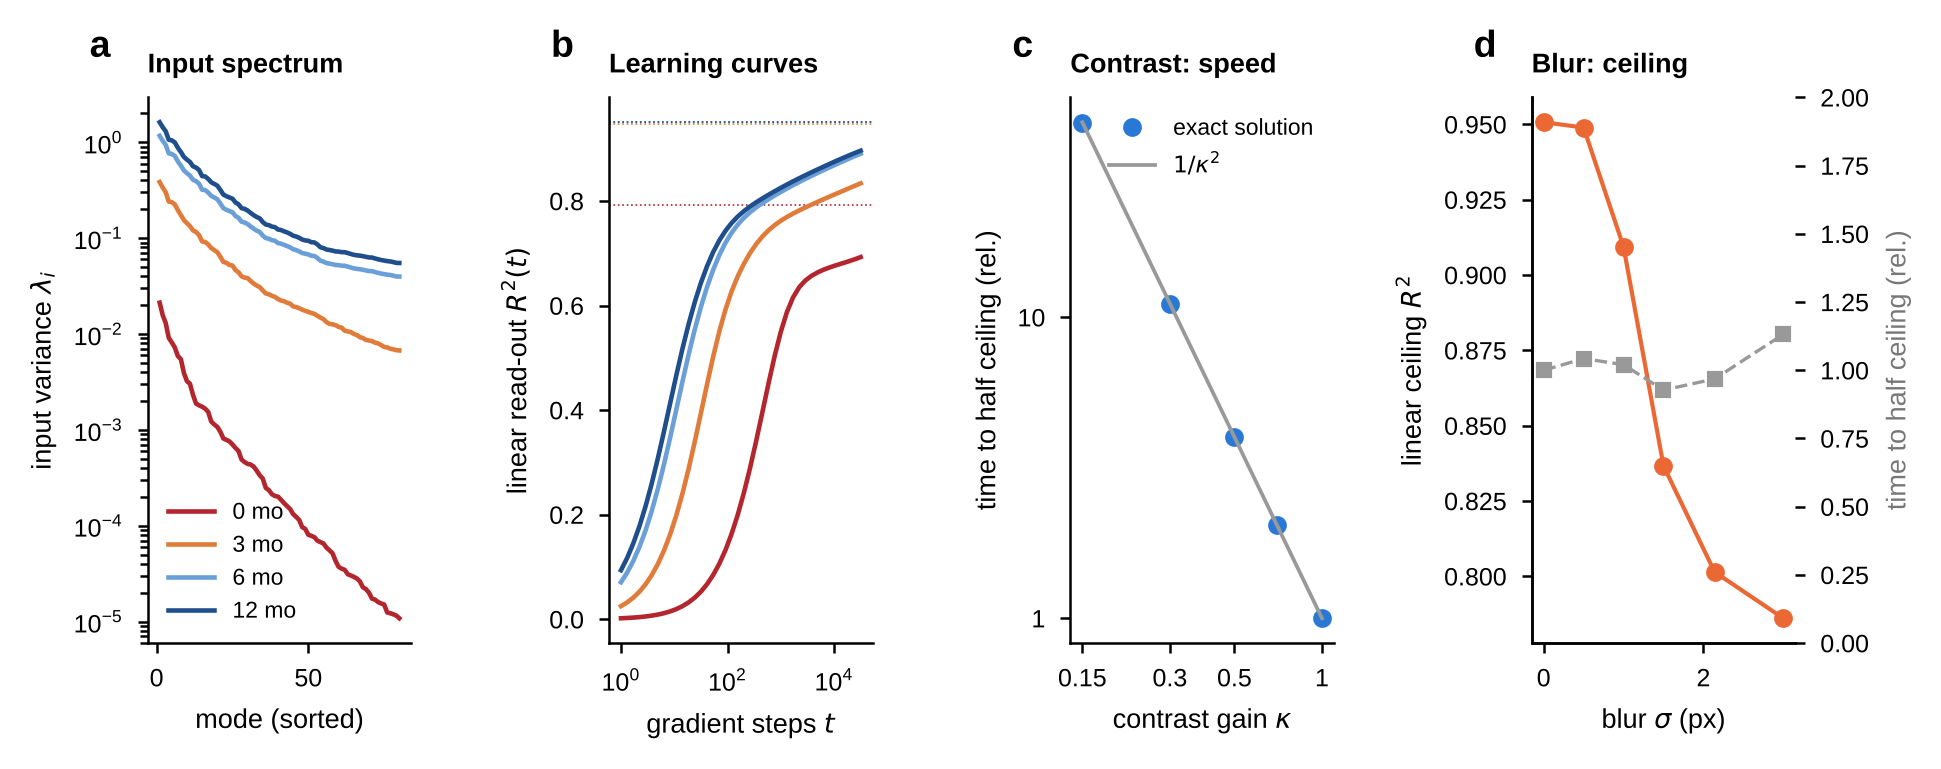
\includegraphics[width=\textwidth,height=0.78\textheight,keepaspectratio]{fig6_theory.png}
\caption{\textbf{Spectral account of learning time.} For the toy-position read-out from filtered frames. \textbf{a}, Eigenvalue spectrum of the input covariance at the four ages: immature front ends shrink it by orders of magnitude. \textbf{b}, Exact gradient-flow solution \(R^2(t)\) of Proposition 2 for each age with the step size fixed by the adult input; dotted lines, the linear ceilings. \textbf{c}, Time to half the ceiling when only contrast is scaled by \(\kappa\): the exact solution follows \(\kappa^{-2}\). \textbf{d}, Blur alone: the ceiling falls with the blur width while the time to half ceiling barely moves.}
\end{figure}


\section{Materials and Methods}

\hypertarget{experimental-design}{%
\subsection{Experimental design}\label{experimental-design}}

The study compares six training regimes (Table 2), plus two front-end ablations for vision, for four sense-specific world models at four checkpoints, with six analyses specified before the final runs: a spectral analysis of the filtered input (below); probes at adult-quality, own-age and newborn-quality input; a supervised information ceiling; violation-of-expectation surprise with dissociating events; occluded tracking and fill-in with a fusion model; and planned statistical comparisons (Table 4). Each regime is trained with the same data, the same number of updates and shared hyperparameters.

\hypertarget{environment}{%
\subsection{Environment}\label{environment}}

Episodes last \(T=20\) frames. A toy of type \(c\in\{1,\dots,4\}\) moves with constant velocity and bounces in a 32\ensuremath{\times}32 scene; the hand's position follows a smoothed random motor command \(u_t\in\mathbb R^2\) and stays in the lower half. Half the episodes contain a vertical screen. Vision is an RGB image on a dark background; the toy is drawn with a type-specific shape and colour, the screen in grey and the hand in skin tone. Hearing is a binaural spectrum, \(o^{\text{aud}}_t\in\mathbb R^{2\times32}\), a Gaussian bump at a type-specific pitch whose loudness falls with distance and whose left/right balance follows horizontal position; sound passes through the screen. Touch is an 8\ensuremath{\times}8 image of the toy's shape when the hand overlaps the toy, otherwise zero. Proprioception is the hand's normalised position and velocity. Ground truth includes toy position, type, visibility and contact. Training sets have 3,000 episodes per seed, test sets 400.

\textbf{Probe events.} \emph{Possible}: the toy crosses a central screen horizontally and reappears. \emph{Impossible}: the toy vanishes while hidden, from every sense. \emph{Vanish-visual}: it vanishes from vision and touch but keeps sounding as if still moving. \emph{Silent}: possible and impossible events with no sound at all (hearing receives noise only). \emph{Track}: like possible, with a wider screen (14 px) and varied speed, so the toy is hidden for about seven frames. Paired events share random draws so that they differ only in the manipulation.

\hypertarget{front-ends}{%
\subsection{Front ends}\label{front-ends}}

All front ends are fixed functions \(\tilde o=\Phi_s(o;a)\) whose parameters are linearly interpolated in age from Table 1.

\emph{Vision.} With acuity \(\mathrm{cpd}(a)\) in cycles per degree, contrast sensitivity \(\mathrm{CS}(a)\) and colour saturation \(\gamma(a)\),
The first equation sets how much to blur the image, with more blur at lower acuity. The equations then apply that blur, pull the contrast towards the image average, and fade the colour towards grey, each by an amount that depends on age.

\begin{equation}\sigma(a)=\tfrac12\cdot\frac{30}{\mathrm{cpd}(a)}\cdot\frac{32}{224},\qquad x=G_{\sigma(a)}*o,\qquad x\leftarrow \bar x+\kappa(a)\,(x-\bar x),\qquad \kappa(a)=\mathrm{clip}\!\left(\tfrac12\log_{10}\mathrm{CS}(a),\,0.15,\,1\right),\end{equation}
\begin{equation}\tilde o=\mathrm{clip}_{[0,1]}\big(\ell+\gamma(a)(x-\ell)\big),\qquad \ell=0.299x_R+0.587x_G+0.114x_B,\end{equation}
where \(G_\sigma\) is a separable Gaussian with replicate padding and \(\bar x\) the image mean. The log compression of contrast replaces a linear gain \(\mathrm{CS}/100\), which would leave a newborn 2\% of contrast; contrast sensitivity is a threshold, not a gain.

\emph{Hearing.} Per ear, \(x=g_{\beta(a)}*o\) along frequency, then a high-frequency roll-off \(x_f\leftarrow x_f\,\mathrm{sigmoid}\big((h(a)\cdot32-f)/1.5\big)\), then reduced interaural difference \(x_{L,R}\leftarrow m+\rho(a)(x_{L,R}-m)\) with \(m=\tfrac12(x_L+x_R)\), then additive Gaussian noise \(\eta(a)\).

\emph{Touch} and \emph{proprioception.} Receptive-field blur \(G_{\tau(a)}\) on the 8\ensuremath{\times}8 patch plus noise; additive noise on proprioception.

\begin{longtable}[]{@{}
  >{\raggedright\arraybackslash}p{(\columnwidth - 8\tabcolsep) * \real{0.2800}}
  >{\raggedright\arraybackslash}p{(\columnwidth - 8\tabcolsep) * \real{0.1800}}
  >{\raggedright\arraybackslash}p{(\columnwidth - 8\tabcolsep) * \real{0.1800}}
  >{\raggedright\arraybackslash}p{(\columnwidth - 8\tabcolsep) * \real{0.1800}}
  >{\raggedright\arraybackslash}p{(\columnwidth - 8\tabcolsep) * \real{0.2000}}@{}}
\caption{Developmental parameters at the four checkpoints (intermediate months are interpolated).}\tabularnewline
\toprule\noalign{}
\begin{minipage}[b]{\linewidth}\raggedright
Sense
\end{minipage} & \begin{minipage}[b]{\linewidth}\raggedright
0 months
\end{minipage} & \begin{minipage}[b]{\linewidth}\raggedright
3 months
\end{minipage} & \begin{minipage}[b]{\linewidth}\raggedright
6 months
\end{minipage} & \begin{minipage}[b]{\linewidth}\raggedright
12 months
\end{minipage} \\
\midrule\noalign{}
\endfirsthead
\toprule\noalign{}
\begin{minipage}[b]{\linewidth}\raggedright
Sense
\end{minipage} & \begin{minipage}[b]{\linewidth}\raggedright
0 months
\end{minipage} & \begin{minipage}[b]{\linewidth}\raggedright
3 months
\end{minipage} & \begin{minipage}[b]{\linewidth}\raggedright
6 months
\end{minipage} & \begin{minipage}[b]{\linewidth}\raggedright
12 months
\end{minipage} \\
\midrule\noalign{}
\endhead
\bottomrule\noalign{}
\endlastfoot
Vision: acuity (cpd) / contrast sensitivity / colour & 1 / 2 / 0.1 & 4 / 10 / 0.7 & 15 / 50 / 1.0 & 30 / 100 / 1.0 \\
Hearing: frequency blur (bins) / high-frequency pass / interaural difference / noise & 2.5 / 60\% / 0.3 / 0.08 & 1.8 / 75\% / 0.5 / 0.06 & 1.0 / 90\% / 0.8 / 0.04 & 0.5 / 100\% / 1.0 / 0.02 \\
Touch: receptive-field blur (taxels) / noise & 1.2 / 0.06 & 0.9 / 0.04 & 0.6 / 0.03 & 0.3 / 0.02 \\
Proprioception: noise & 0.12 & 0.08 & 0.05 & 0.02 \\
Capacity (growing regimes): width multiplier / memory window & \ensuremath{\times}1 / 1 & \ensuremath{\times}2 / 2 & \ensuremath{\times}3 / 4 & \ensuremath{\times}4 / 6 \\
\end{longtable}

\hypertarget{spectral-analysis-and-front-end-ablations}{%
\subsection{Spectral analysis and front-end ablations}\label{spectral-analysis-and-front-end-ablations}}

\textbf{Spectral analysis.} For each age we generated 800 episodes without occluders, kept the 6,000 frames in which the toy is visible, applied the vision front end, centred the pixels and computed the covariance \(\Sigma\) (3,072 \ensuremath{\times} 3,072) and its cross-covariance with the standardised toy position. The closed-form solution of Proposition 2 gives \(R^2(t)\), the linear ceiling \(\sum_i c_i^2/\lambda_i\) (modes with \(\lambda_i<10^{-9}\lambda_{\max}\) are dropped, which acts as a numerical noise floor) and the time to half the ceiling, found by bisection. The step size is fixed at \(1/\lambda_{\max}\) of the adult input so that every age is stable under the same step. We verified the closed form against explicit gradient descent at age 0 (agreement to \(10^{-3}\) in \(R^2\)). Controlled sweeps scale contrast or blur alone at adult quality otherwise. Code: \texttt{scripts/analyze\_spectral.py}; output: \texttt{results/spectral.json}.

\textbf{Front-end ablations.} Two further vision regimes follow the immature schedule for one component of the front end only: \emph{blur only} (acuity follows age, contrast and colour adult) and \emph{contrast only} (contrast sensitivity follows age, acuity and colour adult). All other settings are those of the immature-input regime, with the same seeds.

\hypertarget{sense-world-models}{%
\subsection{Sense world models}\label{sense-world-models}}

For sense \(s\) with latent size \(D_s\) (32 for vision, 16 for hearing and touch, 8 for proprioception),
The encoder \(e\) turns what the sense receives into a short summary \(z_t\). The next summary is the current one plus a correction computed from the last few summaries and the baby's own movement \(u_t\), and the decoder \(d\) turns a summary back into sensory input.

\begin{equation}z_t=e_\theta(\tilde o_t),\qquad \hat z_{t+1}=z_t+f_\theta\big([z_t,z_{t-1},\dots,z_{t-k+1}],u_t\big),\qquad \hat o=d_\theta(z),\end{equation}
where the window is padded with the first frame. The loss on a sub-sequence of 10 frames is
The network is penalised for failing to reproduce what it senses now and for failing to predict what it will sense next, with extra weight on pixels that change, much as babies' eyes are drawn to motion. A small last term keeps the predicted summary close to the real next one.

\begin{equation}\mathcal L=\frac{\sum_t w_t\lVert d(z_t)-\tilde o_t\rVert^2}{\sum_t w_t}+\frac{\sum_t w_{t+1}\lVert d(\hat z_{t+1})-\tilde o_{t+1}\rVert^2}{\sum_t w_{t+1}}+0.1\,\lVert\hat z_{t+1}-\mathrm{sg}(z_{t+1})\rVert^2,\end{equation}
with \(\mathrm{sg}\) the stop-gradient. For vision, per-pixel weights \(w=1+20\,\max_c|\tilde o_t-\tilde o_{t-1}|\) up-weight what moves, a stand-in for the orienting to motion without which the small toy is ignored. The vision encoder is a three-layer CNN with two coordinate channels and the decoder a spatial-broadcast decoder \autocite{watters2019spatial}; other senses use two-layer MLPs. Widths scale with the multiplier \(w\in\{1,2,3,4\}\).

\textbf{Growth.} \texttt{grow(w\textquotesingle{},\ k\textquotesingle{})} widens every hidden layer as in Box 1 and lengthens the window by adding input weights of zero for the new (older) memory slots, so the model's function is unchanged (verified for every layer by a unit test, \texttt{tests/test\_growth.py}). Vision models grow from 43,507 to 586,499 parameters and hearing models from 13,792 to 149,088.

\textbf{Training.} Adam, learning rate \(2\times10^{-3}\), batch 32, 2,000 updates per stage for vision and 1,500 for other senses, four stages in one continuous run; weights carry over between stages and a fresh Adam optimiser is started at each stage, so all regimes see the same optimiser schedule. Hyperparameters were set once on the immature-input regime and shared by all regimes. Seeds: 5 for each regime (fusion uses the grown regime's checkpoints).

\begin{longtable}[]{@{}
  >{\raggedright\arraybackslash}p{(\columnwidth - 4\tabcolsep) * \real{0.3333}}
  >{\raggedright\arraybackslash}p{(\columnwidth - 4\tabcolsep) * \real{0.3333}}
  >{\raggedright\arraybackslash}p{(\columnwidth - 4\tabcolsep) * \real{0.3333}}@{}}
\caption{Training regimes. All see the same episodes for the same number of updates.}\tabularnewline
\toprule\noalign{}
\begin{minipage}[b]{\linewidth}\raggedright
Regime
\end{minipage} & \begin{minipage}[b]{\linewidth}\raggedright
Network
\end{minipage} & \begin{minipage}[b]{\linewidth}\raggedright
Input quality across the four stages
\end{minipage} \\
\midrule\noalign{}
\endfirsthead
\toprule\noalign{}
\begin{minipage}[b]{\linewidth}\raggedright
Regime
\end{minipage} & \begin{minipage}[b]{\linewidth}\raggedright
Network
\end{minipage} & \begin{minipage}[b]{\linewidth}\raggedright
Input quality across the four stages
\end{minipage} \\
\midrule\noalign{}
\endhead
\bottomrule\noalign{}
\endlastfoot
Immature input (primary) & fixed (12-month size) & 0 \ensuremath{\rightarrow} 3 \ensuremath{\rightarrow} 6 \ensuremath{\rightarrow} 12 months \\
Immature input + growth & grows \ensuremath{\times}1 \ensuremath{\rightarrow} \ensuremath{\times}4 & 0 \ensuremath{\rightarrow} 3 \ensuremath{\rightarrow} 6 \ensuremath{\rightarrow} 12 \\
Growth only & grows \ensuremath{\times}1 \ensuremath{\rightarrow} \ensuremath{\times}4 & adult throughout \\
Adult input & fixed & adult throughout \\
Shuffled input quality & fixed & each batch from a random stage \\
Reversed immaturity & fixed & 12 \ensuremath{\rightarrow} 6 \ensuremath{\rightarrow} 3 \ensuremath{\rightarrow} 0 \\
\end{longtable}

\hypertarget{fusion-world-model}{%
\subsection{Fusion world model}\label{fusion-world-model}}

Given frozen sense latents \(z^s_t\) and a mask \(m^s_t\in\{0,1\}\),
The fusion model averages the summaries of whichever senses are available, after mapping each to a common size and tagging it with its sense, and then predicts forward from the last six steps.

\begin{equation}h_t=\mathrm{MLP}\!\left(\frac{\sum_s m^s_t\,(P_s z^s_t+\epsilon_s)}{\max(1,\sum_s m^s_t)}\right),\qquad \hat h_{t+1}=h_t+g\big([h_t,\dots,h_{t-5}],u_t\big),\end{equation}
with projections \(P_s\) to 64 dimensions and learned modality embeddings \(\epsilon_s\). Read-out heads \(r_s\) reconstruct every sense latent from \(h_t\) and from \(\hat h_{t+1}\):
It is trained to recover each sense's own summary from the combined one, both now and one step ahead.

\begin{equation}\mathcal L_{\text{fus}}=\frac1{|S|}\sum_s\Big(\lVert r_s(h_t)-z^s_t\rVert^2+\lVert r_s(\hat h_{t+1})-z^s_{t+1}\rVert^2\Big),\end{equation}
with each sense dropped independently with probability 0.3 during training. Latents are standardised per sense.

\hypertarget{read-outs}{%
\subsection{Read-outs}\label{read-outs}}

\textbf{Linear probes.} For features \(X\) (a latent, or a memory window of latents) and targets \(Y\), ridge regression with centred targets and an unpenalised intercept,
A probe is a straight-line fit from the network's internal state to the quantity of interest, with a small penalty \(\lambda\) against over-fitting; the right-hand expression is its closed-form solution.

\begin{equation}\hat B=\arg\min_B\lVert (Y-\bar Y)-X_cB\rVert^2+\lambda\lVert B\rVert^2=(X_c^\top X_c+\lambda I)^{-1}X_c^\top(Y-\bar Y),\end{equation}
with \(X_c\) standardised features, is fitted on training episodes and evaluated on test episodes, \(R^2=1-\sum\lVert y-\hat y\rVert^2/\sum\lVert y-\bar y\rVert^2\). Identity uses one-hot targets and the arg-max (chance 0.25). Touch is probed on contact frames, proprioception on hand position. \emph{Adult-input} probes use adult-quality input; \emph{own-age} probes use the input quality of the checkpoint's age; \emph{newborn-input} probes are fitted on adult-quality input and tested on newborn-quality input.

\textbf{Information ceiling.} For each sense and age \(a\in\{0,1,2,3,4,6,9,12\}\), a supervised network (the same encoder family) is trained for 1,500 updates to predict toy position and identity from a single filtered frame, and evaluated on held-out frames.

\textbf{Violation of expectation.} Surprise is one-step prediction error, \(S_t=\lVert d(\hat z_t)-\tilde o_t\rVert^2\) (unimodal) or \(\lVert r_s(\hat h_t)-z^s_t\rVert^2\) per channel (fused, standardised latents), averaged over the hidden stretch and the two frames after expected re-emergence. With \(S_{\text{pos}}\) and \(S_{\text{imp}}\) the mean surprise on paired possible and impossible events,
The first quantity balances surprise at the impossible event against surprise at the possible one. It runs from \(-1\), when only the possible event surprises, through 0, when both do equally, to \(+1\), when only the impossible one does. The second is the average difference divided by its spread across episodes.

\begin{equation}\mathrm{VoE}=\frac{S_{\text{imp}}-S_{\text{pos}}}{S_{\text{imp}}+S_{\text{pos}}},\qquad d_z=\frac{\overline{S_{\text{imp}}-S_{\text{pos}}}}{\mathrm{sd}(S_{\text{imp}}-S_{\text{pos}})}.\end{equation}

\textbf{Occluded tracking and fill-in.} The hidden toy's horizontal position is probed on fully hidden frames of the \emph{track} events from the vision model's memory window (\(k=6\) latents), from the hearing latent, and from the fused state, fitting on half of the episodes and testing on the other half. Fill-in probes toy position from the fused state with all senses, without vision, and from single senses.

\textbf{Statistics.} Bands and whiskers are \ensuremath{\pm}1 s.d. over seeds. Planned comparisons at the 12-month checkpoint use Welch's t-test and Hedges' \(g=\frac{\bar a-\bar b}{s_p}\big(1-\frac{3}{4(n_a+n_b)-9}\big)\) with approximate 95\% interval \(g\pm1.96\sqrt{\frac{n_a+n_b}{n_an_b}+\frac{g^2}{2(n_a+n_b)}}\); per-cell 95\% bootstrap intervals are in \texttt{results/extra.json}. No correction for multiple comparisons is applied; we list all planned comparisons.

\begin{longtable}[]{@{}llll@{}}
\caption{Planned comparisons.}\tabularnewline
\toprule\noalign{}
Comparison (12-month checkpoint) & Hedges' g & p (Welch) & n \\
\midrule\noalign{}
\endfirsthead
\toprule\noalign{}
Comparison (12-month checkpoint) & Hedges' g & p (Welch) & n \\
\midrule\noalign{}
\endhead
\bottomrule\noalign{}
\endlastfoot
Vision clean, immature vs adult input & \ensuremath{-}1.2 & 0.06 & 5/5 \\
Vision clean, grown vs immature & \ensuremath{-}1.0 & 0.11 & 5/5 \\
Vision identity, grown vs immature & \ensuremath{-}2.2 & 0.005 & 5/5 \\
Vision on newborn input, immature vs adult & 0.9 & 0.16 & 5/5 \\
Hearing clean, immature vs adult & 1.5 & 0.05 & 5/5 \\
Hearing clean, grown vs growth only & 1.6 & 0.05 & 5/5 \\
Hidden toy, fused vs vision memory & 1.8 & 0.01 & 5/5 \\
\end{longtable}

\textbf{Compute.} Training compute is approximated by \(\sum_{\text{stages}}(\text{parameters})\times(\text{updates})\); relative to a fixed 12-month-size network, grown vision models use 0.48 and grown hearing models 0.49.

\textbf{Milestones.} For each sense, the half-ceiling age is the first age at which the ceiling reaches half of its 12-month value (position R\textsuperscript{2} for vision and hearing; identity accuracy above chance for touch). Kendall's \ensuremath{\tau} compares the resulting order with the order of functional maturity usually described for the three senses, touch before hearing before vision \autocite{turkewitz1982limitations}.

\textbf{Human and animal studies.} The study uses only synthetic data; no human or animal participants were involved.

\textbf{Code and data availability.} All code, configurations, results and trained checkpoints are at \url{https://github.com/pikulsomesh/developmental-world-models} (MIT licence). \texttt{scripts/run\_experiments.py} trains every regime, \texttt{scripts/analyze\_fusion\_voe.py} and \texttt{scripts/analyze\_extra.py} run the analyses, \texttt{scripts/make\_paper\_figures.py} draws the figures, and \texttt{scripts/fill\_report.py} writes every number in this report from the results files. An interactive companion and wiki are at \url{https://pikulsomesh.github.io/developmental-world-models/}.


\section{Results}

\hypertarget{a-simulation-that-isolates-each-constraint}{%
\subsection{A simulation that isolates each constraint}\label{a-simulation-that-isolates-each-constraint}}

The simulated world renders one toy of four types, a babbling hand and, in half the scenes, a vertical screen into four streams: 32\ensuremath{\times}32 colour vision, binaural hearing (2 ears \ensuremath{\times} 32 frequency bins, panned by position and passing through the screen), an 8\ensuremath{\times}8 tactile patch on the hand, and four-dimensional proprioception (Fig. 1a; Methods). Each toy type is specified redundantly across senses, by shape and colour, pitch and felt shape \autocite{bahrick2000intersensory}. Each sense is filtered by a fixed front end whose parameters follow the age \(a\) (Fig. 1b, c; Table 1); for vision the parameters are published infant acuity and contrast sensitivity \autocite{norcia1985spatial,banks1988optical}, and for hearing, touch and proprioception they are coarse placeholder tables that respect the known order of maturation. Behind each front end is a world model of the same family (Methods). Each sense is trained in one continuous run of four stages and read out at the end of each. Six regimes (Fig. 1d; Table 2) cross the two levers, input schedule and network growth, with two order controls.

\begin{figure}[tbp]
\centering
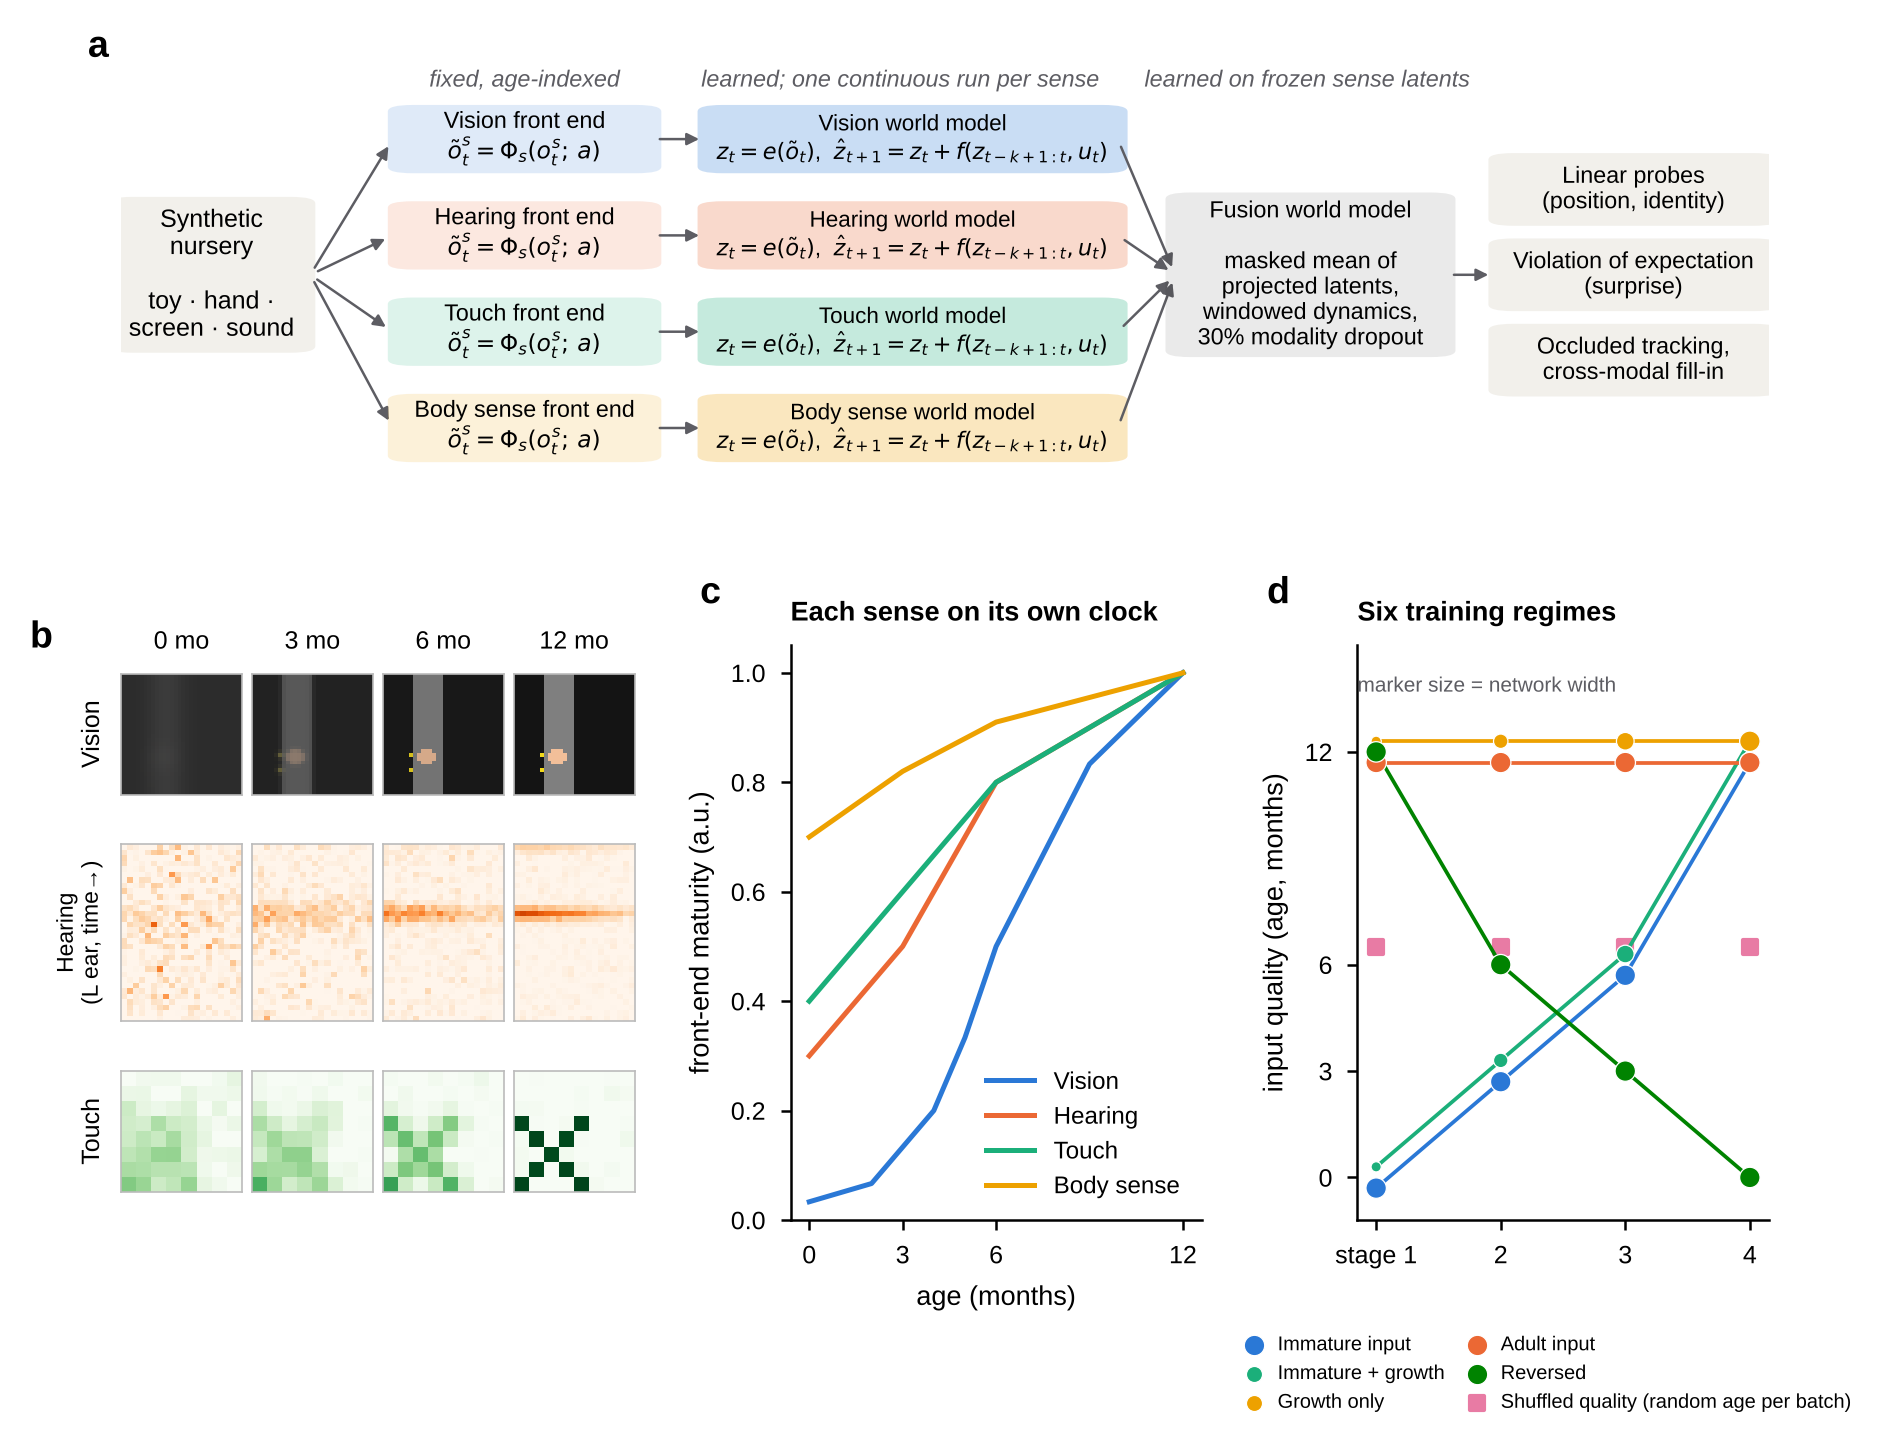
\includegraphics[width=\textwidth,height=0.78\textheight,keepaspectratio]{fig1_overview.png}
\caption{\textbf{Sense-specific developmental world models.} \textbf{a}, Each sense passes a synthetic nursery (a toy that is seen, heard and felt, the infant's babbling hand, and an occluding screen) through a fixed, age-indexed front end \(\Phi_s(\cdot;a)\), and learns its own world model: an encoder \(e\), a dynamics model \(f\) over the last \(k\) latents and the infant's motor command \(u_t\), and a decoder. A fusion world model combines the frozen sense latents. Read-outs are linear probes, violation-of-expectation surprise and occluded tracking. \textbf{b}, The same moment delivered to vision, hearing (left ear, 32 frequency bins over the episode) and touch (an 8\ensuremath{\times}8 patch of skin) at 0, 3, 6 and 12 months. \textbf{c}, Front-end maturity per sense (normalised parameters of Table 1): touch and proprioception start close to mature, hearing partly, vision far behind. \textbf{d}, The six training regimes: input quality over the four training stages; marker size is network width.}
\end{figure}

\hypertarget{the-input-sets-the-order-of-development-and-learning-lags-what-the-input-allows}{%
\subsection{The input sets the order of development, and learning lags what the input allows}\label{the-input-sets-the-order-of-development-and-learning-lags-what-the-input-allows}}

\begin{figure}[tbp]
\centering
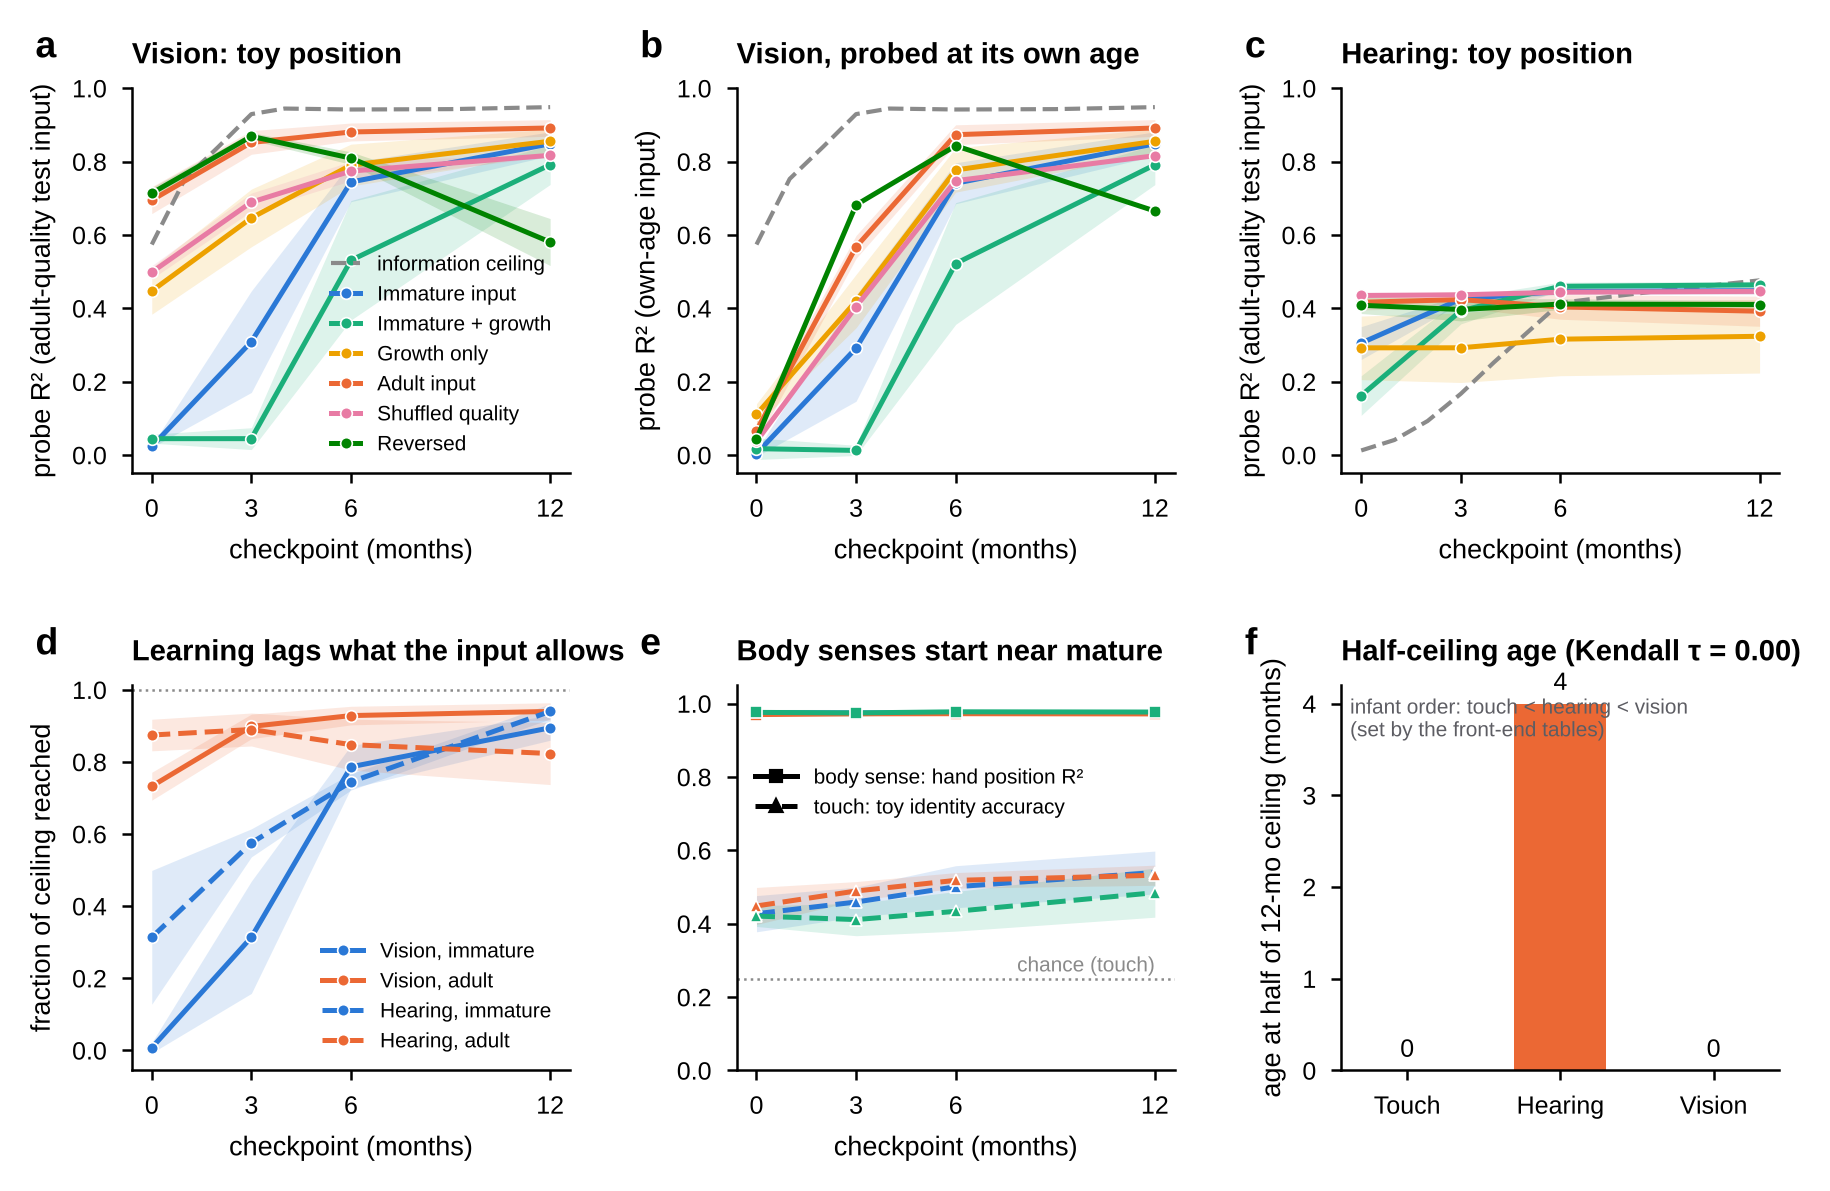
\includegraphics[width=\textwidth,height=0.78\textheight,keepaspectratio]{fig2_development.png}
\caption{\textbf{Development of each sense.} \textbf{a}, Toy position decoded from the vision model's latent at each checkpoint (probe fitted and tested on adult-quality input), for the six regimes; dashed grey line, information ceiling (a supervised network trained directly on that age's filtered input). \textbf{b}, The same with the probe fitted and tested on the input quality of the checkpoint's own age. \textbf{c}, Hearing. \textbf{d}, Fraction of the age-matched ceiling reached by the immature-input regime (own-age probe) and by the adult-input regime, for vision (solid) and hearing (dashed). \textbf{e}, Proprioception (hand position R\textsuperscript{2}, squares) and touch (toy identity accuracy, triangles; chance 0.25) are close to their final level from the first checkpoint. \textbf{f}, Age at which each sense's information ceiling first reaches half its 12-month value; this measure does not recover the infant order (Kendall \ensuremath{\tau} against touch \textless{} hearing \textless{} vision in the panel title), because the vision ceiling is already high at birth. Lines, mean over seeds; bands, \ensuremath{\pm}1 s.d.; n = 5 seeds per regime.}
\end{figure}

With immature input, the vision model cannot localise the toy at the first checkpoint (position \(R^2\) 0.02 \ensuremath{\pm} 0.00) and is still poor at the second (0.31 \ensuremath{\pm} 0.15), then rises to 0.85 \ensuremath{\pm} 0.04 (Fig. 3a). Trained on adult-quality input the same network localises the toy from the first checkpoint (0.69 \ensuremath{\pm} 0.04) and ends at 0.89 \ensuremath{\pm} 0.03. Hearing, touch and the body senses are close to their final level much earlier (Fig. 3c, e), so vision is the last sense to develop, which is put there by the front-end tables. Measured by the age at which each sense's information ceiling reaches half its 12-month value (touch 0, hearing 4, vision 0 months; Kendall \(\tau\) = 0.00 against the order touch, hearing, vision; Fig. 3f) the infant order is not recovered, because the vision ceiling is already high at birth even though the learned model is not.

Proposition 1 asks whether this early failure is the input or the learner. Probing on each checkpoint's own input (Fig. 3b) gives 0.00 \ensuremath{\pm} 0.01 at 0 months and 0.85 \ensuremath{\pm} 0.04 at 12, so it is not a distribution shift from training on blurred and testing on sharp images. The newborn input is not empty: a supervised network trained directly on it reaches \(R^2\) = 0.57 (Fig. 3a, dashed), and the exact linear solution of Proposition 2 reaches 0.79. The gap between 0.57 and 0.02 is therefore a property of learning. Proposition 2 also quantifies it: with the step size set by adult input, the newborn front end shrinks the total input variance from 32.20 to 0.12 and lengthens the time to half ceiling 39-fold (Fig. 2a, b). The vision model approaches its ceiling only as the front end sharpens (Fig. 3d).

\hypertarget{contrast-sets-the-speed-of-learning-and-blur-sets-the-ceiling-in-theory-and-in-the-linear-model}{%
\subsection{Contrast sets the speed of learning and blur sets the ceiling, in theory and in the linear model}\label{contrast-sets-the-speed-of-learning-and-blur-sets-the-ceiling-in-theory-and-in-the-linear-model}}

Scaling contrast alone by \(\kappa\) delays the linear solution by \(\kappa^{-2}\) to within 1\% over a 44-fold range, and leaves its ceiling unchanged (Fig. 2c). Blur alone leaves the time to half ceiling almost unchanged but lowers the ceiling from 0.95 without blur to 0.80 at the newborn width of 2.14 px (Fig. 2d). The linear read-out is not the network, and the networks are trained with Adam, which removes the global scale effect; ablations of the front end test which component matters in the trained vision model.

ABLATION\_SECTION\_PENDING

\hypertarget{growth-delays-learning-and-halves-the-parameter-updates}{%
\subsection{Growth delays learning and halves the parameter-updates}\label{growth-delays-learning-and-halves-the-parameter-updates}}

Adding growth to immature input does not change the shape of the curve; it delays it (Fig. 3a). The grown vision model is still at \(R^2\) 0.04 \ensuremath{\pm} 0.03 at the 3-month checkpoint and ends at 0.79 \ensuremath{\pm} 0.06, against 0.85 \ensuremath{\pm} 0.04 for the fixed-size network; identity accuracy is 0.49 \ensuremath{\pm} 0.06 against 0.64 \ensuremath{\pm} 0.06 (Hedges' \(g\) = \ensuremath{-}2.2, \(p\) = 0.005). Growth without immature input learns quickly and ends near the adult-input model (0.86 \ensuremath{\pm} 0.04). At matched updates, growing networks use 0.48 of the fixed network's parameter-updates (Fig. 5d). This is the plateau Proposition 3 predicts: new units begin learning only through their outgoing weights, so each widening is followed by a stall, and growth trades accuracy for compute.

\hypertarget{early-immaturity-costs-vision-a-little-and-helps-hearing}{%
\subsection{Early immaturity costs vision a little and helps hearing}\label{early-immaturity-costs-vision-a-little-and-helps-hearing}}

\begin{figure}[tbp]
\centering
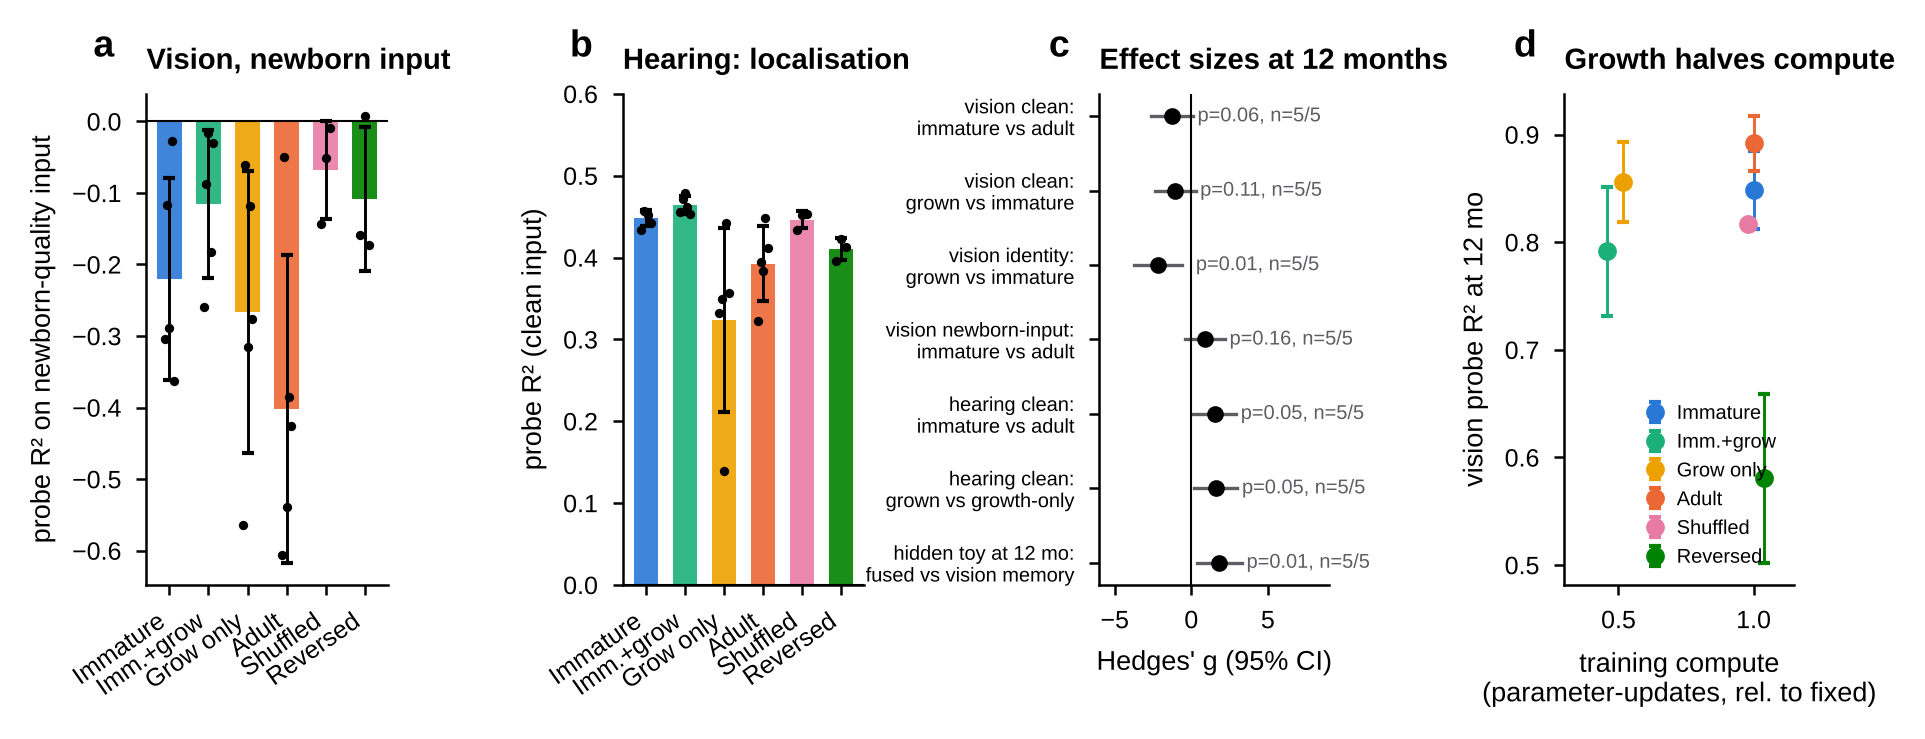
\includegraphics[width=\textwidth,height=0.78\textheight,keepaspectratio]{fig3_costs_benefits.png}
\caption{\textbf{Costs and benefits at the 12-month checkpoint.} \textbf{a}, Vision probe R\textsuperscript{2} when tested on newborn-quality input (bars, mean; dots, seeds; whiskers, s.d.). All values are negative (worse than predicting the mean), so differences are in how badly models fail. \textbf{b}, Hearing localisation on clean input. \textbf{c}, Effect sizes (Hedges' g with approximate 95\% CI) and Welch-test p values for the planned comparisons; n per group shown. \textbf{d}, Vision accuracy against training compute (parameter-updates relative to a fixed-size network).}
\end{figure}

On clean input the adult-input vision model is best. Immature input costs 0.89 \ensuremath{-} 0.85 in \(R^2\) (\(g\) = \ensuremath{-}1.2, \(p\) = 0.06). Tested on newborn-quality input, every model fails (Fig. 5a), with regimes that saw immature input failing less on average (\ensuremath{-}0.22 \ensuremath{\pm} 0.14 against \ensuremath{-}0.40 \ensuremath{\pm} 0.22 for adult input), but the difference is within seed variability (\(p\) = 0.16); we do not claim a robustness benefit in vision.

Hearing differs. Models that heard immature sound early localise better on clean input at 12 months (0.45 \ensuremath{\pm} 0.01 immature, 0.46 \ensuremath{\pm} 0.01 immature with growth) than models that only heard adult-quality sound (0.39 \ensuremath{\pm} 0.05 adult input, 0.32 \ensuremath{\pm} 0.11 growth only; Fig. 5b; \(g\) = 1.5, \(p\) = 0.05). Shuffled input quality (0.45 \ensuremath{\pm} 0.01) is close to the immature schedule, so the benefit comes from having heard degraded input at all, a form of augmentation (the mixture objective of training at several qualities), more than from its order. Reversing the schedule is the clearest negative control: the vision model that ends on newborn-quality input falls from 0.87 \ensuremath{\pm} 0.01 to 0.58 \ensuremath{\pm} 0.08, so what the model has learned does not survive a late degradation.

\hypertarget{fusing-senses-recovers-what-each-sense-alone-loses}{%
\subsection{Fusing senses recovers what each sense alone loses}\label{fusing-senses-recovers-what-each-sense-alone-loses}}

\begin{figure}[tbp]
\centering
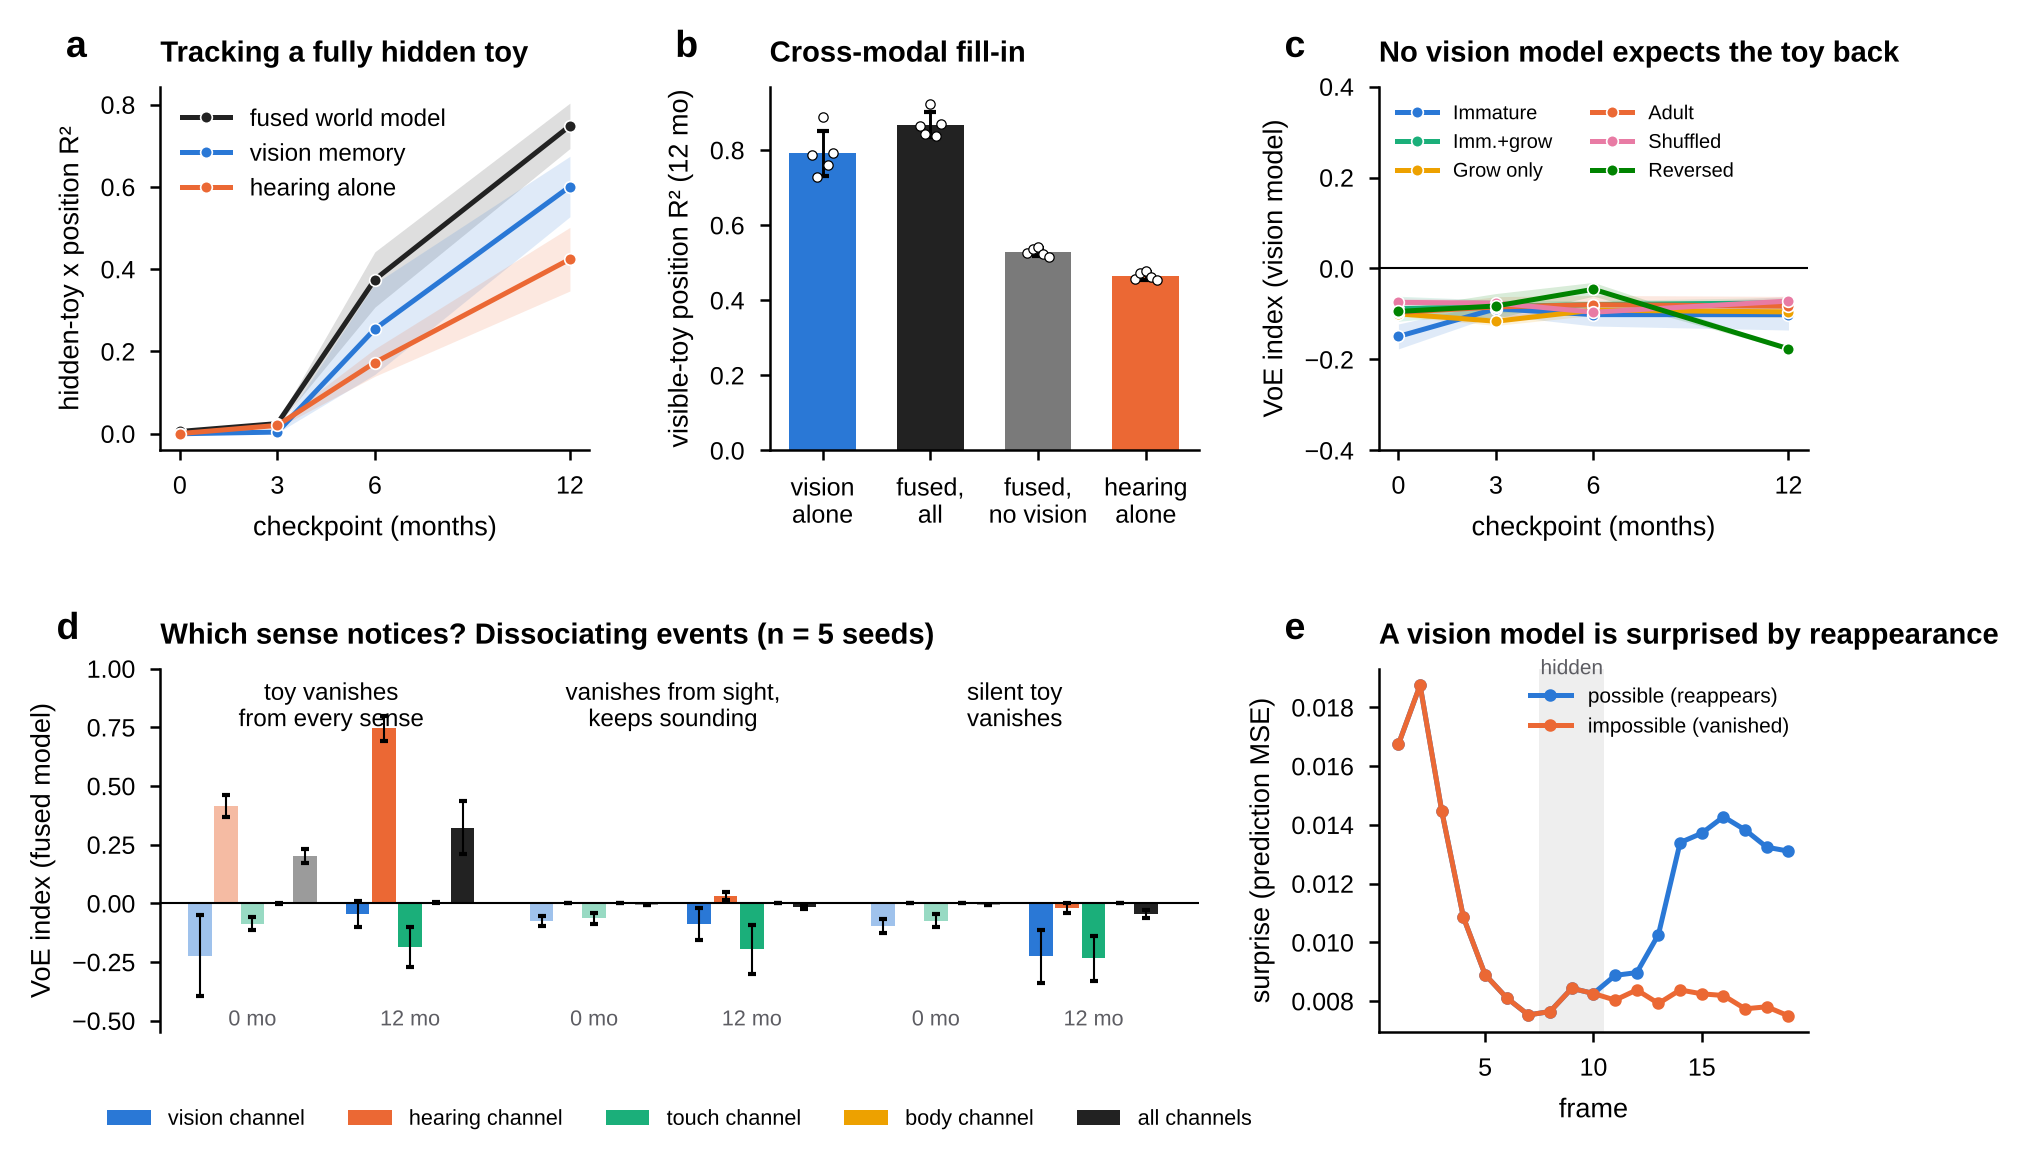
\includegraphics[width=\textwidth,height=0.78\textheight,keepaspectratio]{fig4_fusion_expectation.png}
\caption{\textbf{Fusion and expectation.} \textbf{a}, Horizontal position of a fully hidden toy decoded from the vision model's memory window, from hearing alone and from the fused world model. \textbf{b}, Position of a visible toy at 12 months from vision alone, the fused state, the fused state with vision switched off, and hearing alone. \textbf{c}, Violation-of-expectation (VoE) index of the unimodal vision models; positive means more surprise when the toy fails to reappear. \textbf{d}, VoE index of the fused model broken down by channel, for three events: the toy vanishes from every sense; it vanishes from sight and touch but keeps sounding; a silent toy vanishes. Faded bars, 0 months; solid, 12 months. \textbf{e}, Frame-by-frame surprise of one vision model (immature input, 12 months) on a possible and an impossible event; grey, toy hidden. Bands and whiskers, \ensuremath{\pm}1 s.d. over seeds.}
\end{figure}

During a long occlusion, the hidden toy's horizontal position can be decoded from the vision model's memory (\(R^2\) 0.60 \ensuremath{\pm} 0.08 at 12 months), from hearing, which passes through the screen (0.42 \ensuremath{\pm} 0.09), and best from the fused world model (0.75 \ensuremath{\pm} 0.06; Fig. 6a; paired difference fused minus vision positive in every seed). The advantage appears at 6 months and nothing is decodable at 0 to 3 months, when neither vision nor binaural hearing can localise. For a visible toy, the fused state is better than vision alone (0.87 \ensuremath{\pm} 0.03 against 0.79 \ensuremath{\pm} 0.06) and, with vision switched off, still recovers position from hearing, touch and the hand (0.53 \ensuremath{\pm} 0.01; Fig. 6b).

\hypertarget{surprise-follows-the-conditional-mean-not-the-stored-position}{%
\subsection{Surprise follows the conditional mean, not the stored position}\label{surprise-follows-the-conditional-mean-not-the-stored-position}}

No unimodal vision model, in any regime, has a positive violation-of-expectation index (Fig. 6c): all are more surprised when the toy reappears than when it fails to, like a predictor that copies the last frame (Fig. 6e). This holds although the hidden toy's position is decodable from the same model's memory. It is the behaviour Proposition 4 predicts for a squared-error forecaster when the reappearance time is uncertain.

The fused model does show a positive index when the toy vanishes from every sense (0.32 \ensuremath{\pm} 0.11 at 12 months), but its channels show where the surprise comes from: hearing 0.75 \ensuremath{\pm} 0.05, vision \ensuremath{-}0.04 \ensuremath{\pm} 0.05 (Fig. 6d). The model notices that the sound stopped. When the toy vanishes from sight but keeps sounding, the overall index is \ensuremath{-}0.02 \ensuremath{\pm} 0.01 and the vision channel \ensuremath{-}0.09 \ensuremath{\pm} 0.07; when a silent toy vanishes, they are \ensuremath{-}0.04 \ensuremath{\pm} 0.02 and \ensuremath{-}0.23 \ensuremath{\pm} 0.11. Without a sound to give the event away, the fused model does not expect the toy back either: a read-out can show that information about a hidden object is present while the model's predictions do not use it.


\section{Discussion}

\textbf{What the theory explains.} Table 3 sets each proposition against what we observed. The information bound and the learning-time law together account for the main shape of development in the vision model: a front end that shrinks input variance and removes fine detail makes the early read-out both lower and slower, and the self-supervised model reaches only a small fraction of the ceiling until the front end sharpens. The growth delay accounts for why growing the network did not help, and the conditional-mean result accounts for the sign of the surprise index.

\begin{longtable}[]{@{}
  >{\raggedright\arraybackslash}p{(\columnwidth - 4\tabcolsep) * \real{0.3333}}
  >{\raggedright\arraybackslash}p{(\columnwidth - 4\tabcolsep) * \real{0.3333}}
  >{\raggedright\arraybackslash}p{(\columnwidth - 4\tabcolsep) * \real{0.3333}}@{}}
\caption{Predictions of the theory and what was observed.}\tabularnewline
\toprule\noalign{}
\begin{minipage}[b]{\linewidth}\raggedright
Proposition
\end{minipage} & \begin{minipage}[b]{\linewidth}\raggedright
Prediction
\end{minipage} & \begin{minipage}[b]{\linewidth}\raggedright
Observation
\end{minipage} \\
\midrule\noalign{}
\endfirsthead
\toprule\noalign{}
\begin{minipage}[b]{\linewidth}\raggedright
Proposition
\end{minipage} & \begin{minipage}[b]{\linewidth}\raggedright
Prediction
\end{minipage} & \begin{minipage}[b]{\linewidth}\raggedright
Observation
\end{minipage} \\
\midrule\noalign{}
\endhead
\bottomrule\noalign{}
\endlastfoot
1. Information bound & Learned score cannot exceed the ceiling at that input quality & Holds at every age; early gap is large for vision \\
2. Learning time & Contrast scales speed by \(\kappa^{-2}\); blur limits the ceiling & Exact in the linear model; trained-network ablations in Results \\
3. Growth delay & A plateau after each widening; fewer parameter-updates & Grown model lags; uses about half the parameter-updates \\
4. Conditional mean & Negative surprise index when reappearance is uncertain & Negative for every unimodal vision model; positive only when a sound gives the event away \\
\end{longtable}

\textbf{What it does not explain.} The linear solution is a lower bound on how deep networks behave, and the trained vision model lags its ceiling far more than the linear model lags its own, which shows that most of the delay lies in learning features, not in fitting a read-out. Proposition 2 does not apply as stated to adaptive optimisers, and the ablations show which component of the front end matters in practice. Nor does the theory explain the benefit of early immaturity in hearing: the shuffled-order control suggests augmentation, but we have not derived it.

\textbf{Implications for staged training.} Three design rules follow, each stated for the setting studied here. Reduce contrast or gain only if the cost in speed is acceptable, because it delays learning by the square of the scale with plain gradient descent and gives no lasting information benefit; use blur when the aim is to withhold fine detail early, and expect a lower ceiling in a finite budget; and do not use growth as a substitute for a schedule, because new units contribute nothing until their outgoing weights move. When surprise is the read-out, a squared-error pixel forecaster is the wrong instrument: objectives that predict in latent space \autocite{garrido2025intuitive}, represent uncertainty explicitly or are trained on longer horizons should be tested against the same dissociating events.

\textbf{Limitations.} Everything is synthetic and small (at most 0.6 million parameters per sense) and is evaluated mainly with linear probes, which measure decodability, not behaviour. The theory is exact for a linear read-out under gradient flow and is suggestive for trained networks. Hearing, touch and proprioception tables are placeholders, and ``months'' are training stages, not hours of experience. With 5 seeds per regime, several comparisons have large effect sizes but are not significant (Fig. 5c); we report them as estimates. An internal referee report and our responses are provided with the code (\texttt{papers/world-models/report/PEER\_REVIEW.md}).

\textbf{Future work.} The immediate extensions are experience-matched checkpoints of one continuous run per sense, late fusion with sense-onset order as a factor, latent-space and uncertainty-aware objectives tested against the dissociating events, and extending the spectral account to deep networks by measuring the singular-value spectrum of the learned input-output map. The data path runs from this synthetic simulation to an embodied simulator for touch and proprioception \autocite{mattern2024mimo} and to head-camera corpora for vision and hearing \autocite{sullivan2021saycam,long2024babyview}.


\textbf{General.} During the preparation of this work, the author used an AI assistant (Claude, Anthropic) to help write and run analysis code, draw figures and draft text. The author reviewed and edited the content and takes full responsibility for the content of the publication.

\textbf{Author contributions.} S. Mohapatra conceived the study, directed the work and approved the final text.

\textbf{Funding.} This work received no specific funding and was carried out independently.

\textbf{Competing interests.} The author declares that there is no conflict of interest regarding the publication of this article.

\textbf{Data availability.} All code, configurations, aggregated results and trained checkpoints are available at github.com/pikulsomesh/developmental-world-models. The data are synthetic and are regenerated by the code from the random seeds listed in the repository.

Extended Data Figs. 1 to 3 (below), \texttt{report/REFERENCES\_VERIFIED.md} (the reference-verification log) and \texttt{papers/world-models/report/PEER\_REVIEW.md} (an internal referee report with responses) are available in the repository.

\clearpage
\section*{Extended Data (Supplementary Figures)}
\setcounter{figure}{0}
\renewcommand{\thefigure}{S\arabic{figure}}

\begin{figure}[tbp]
\centering
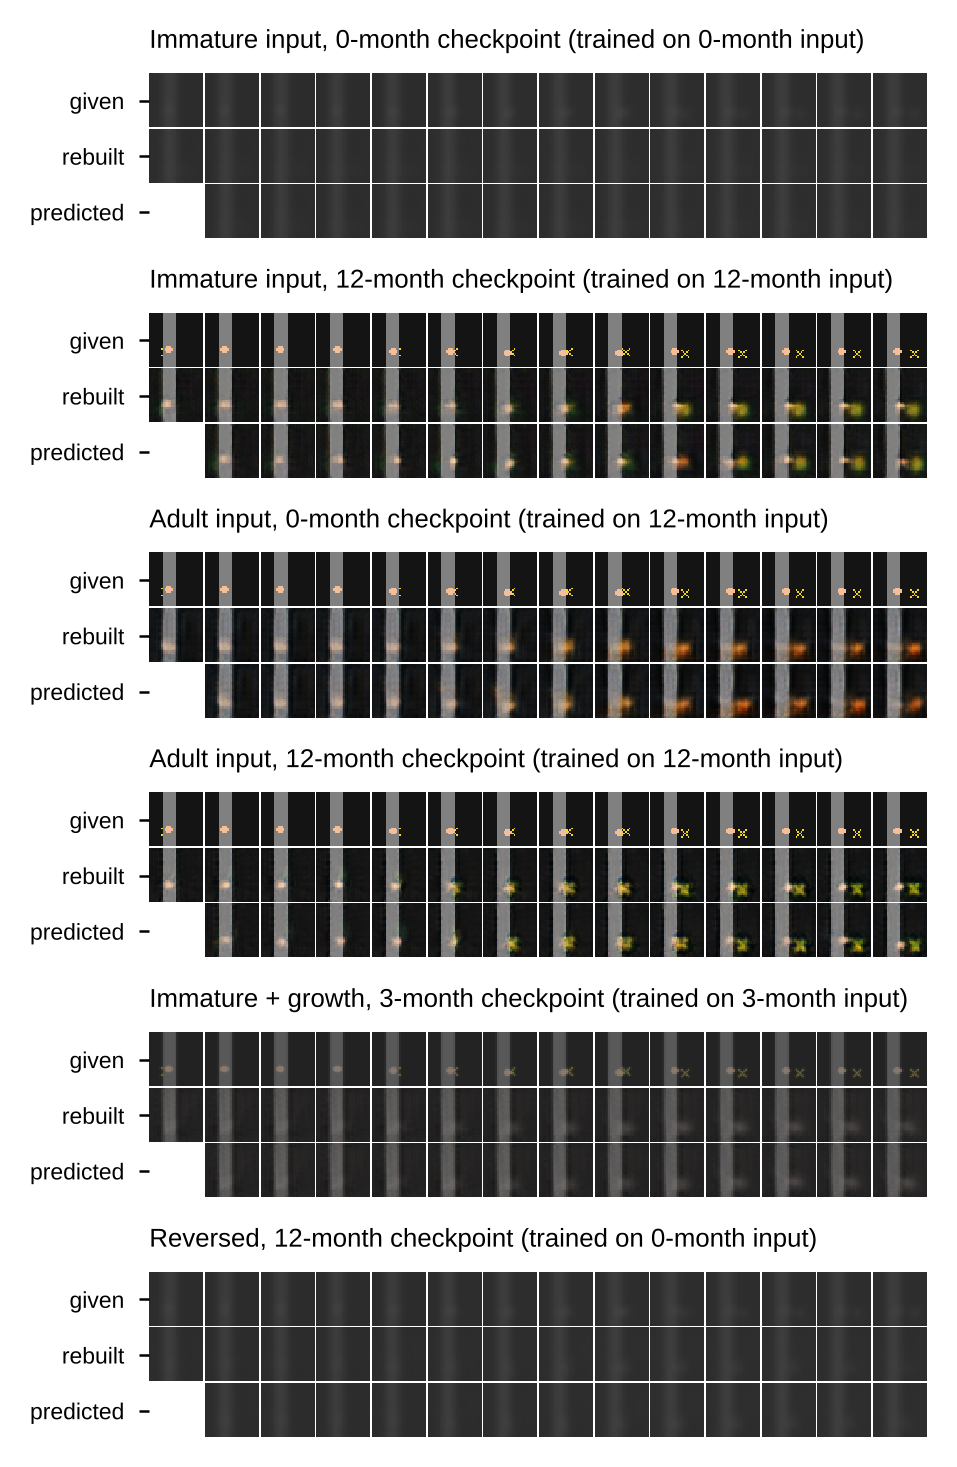
\includegraphics[width=\textwidth,height=0.78\textheight,keepaspectratio]{ed1_model_outputs.png}
\caption{\textbf{What the vision models see, rebuild and predict.} For selected regimes and checkpoints: the input given (at the age that stage was trained on), the reconstruction from the latent, and the one-step prediction, for the first 14 frames of one episode.}
\end{figure}

\begin{figure}[tbp]
\centering
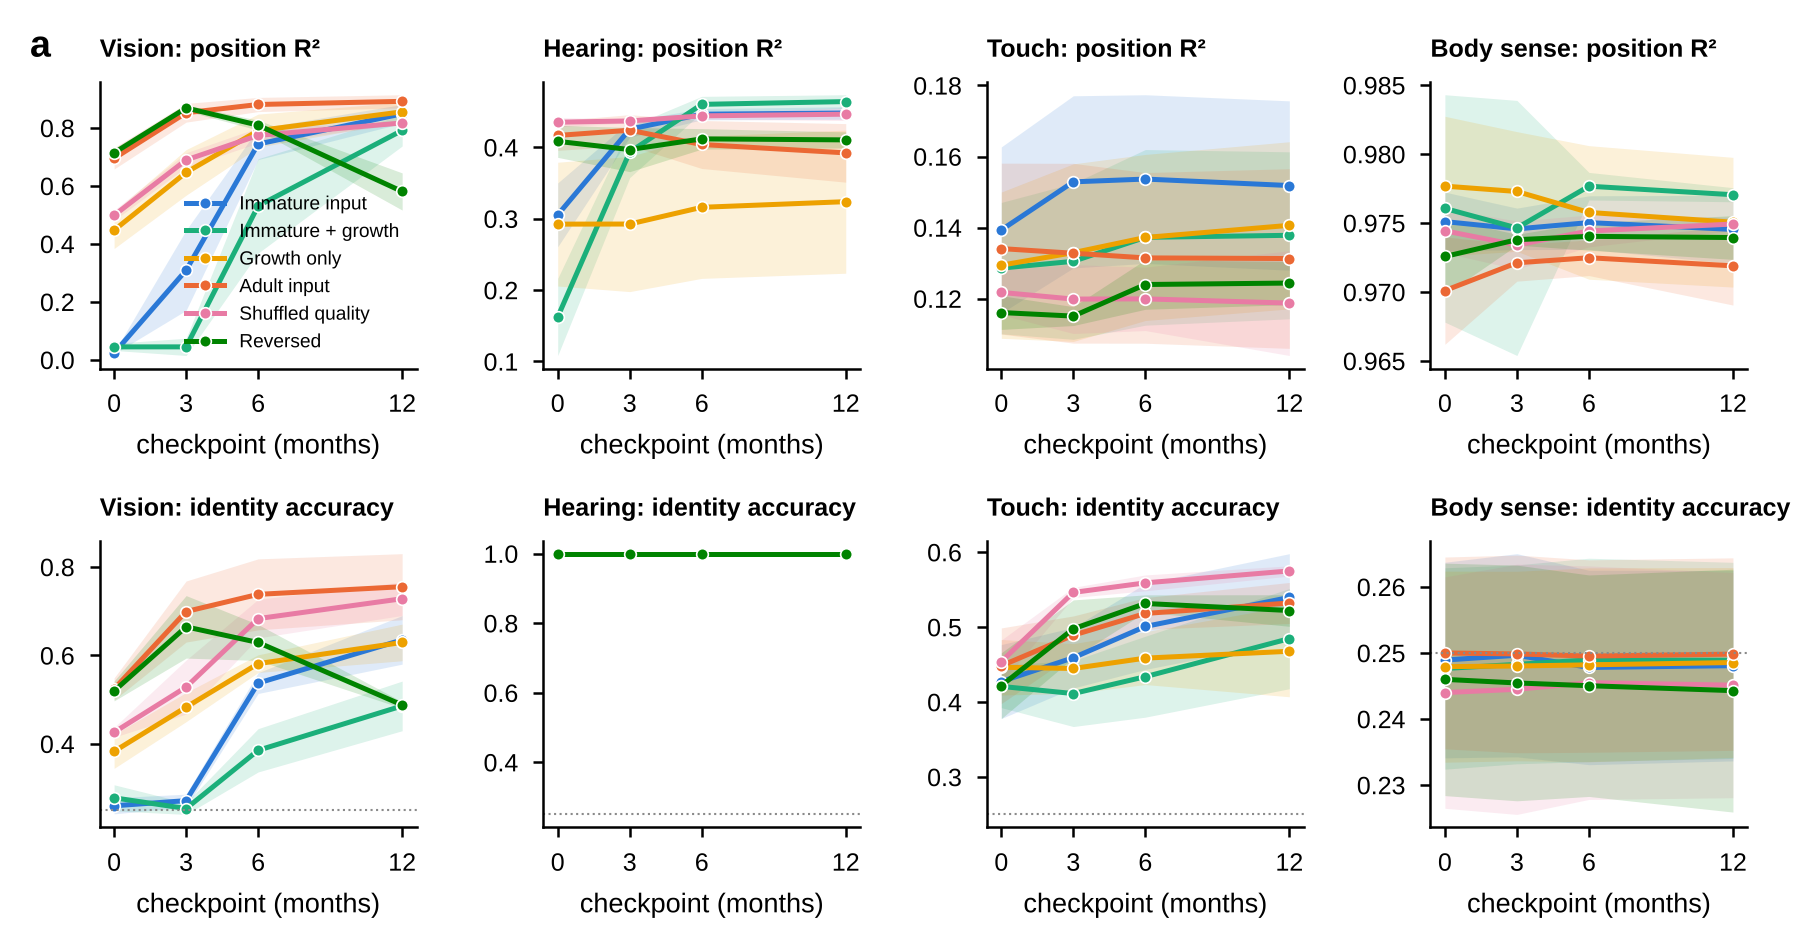
\includegraphics[width=\textwidth,height=0.78\textheight,keepaspectratio]{ed2_all_senses.png}
\caption{\textbf{All senses, all regimes.} Position R\textsuperscript{2} (top) and identity accuracy (bottom; dotted, chance) per checkpoint.}
\end{figure}

\begin{figure}[tbp]
\centering
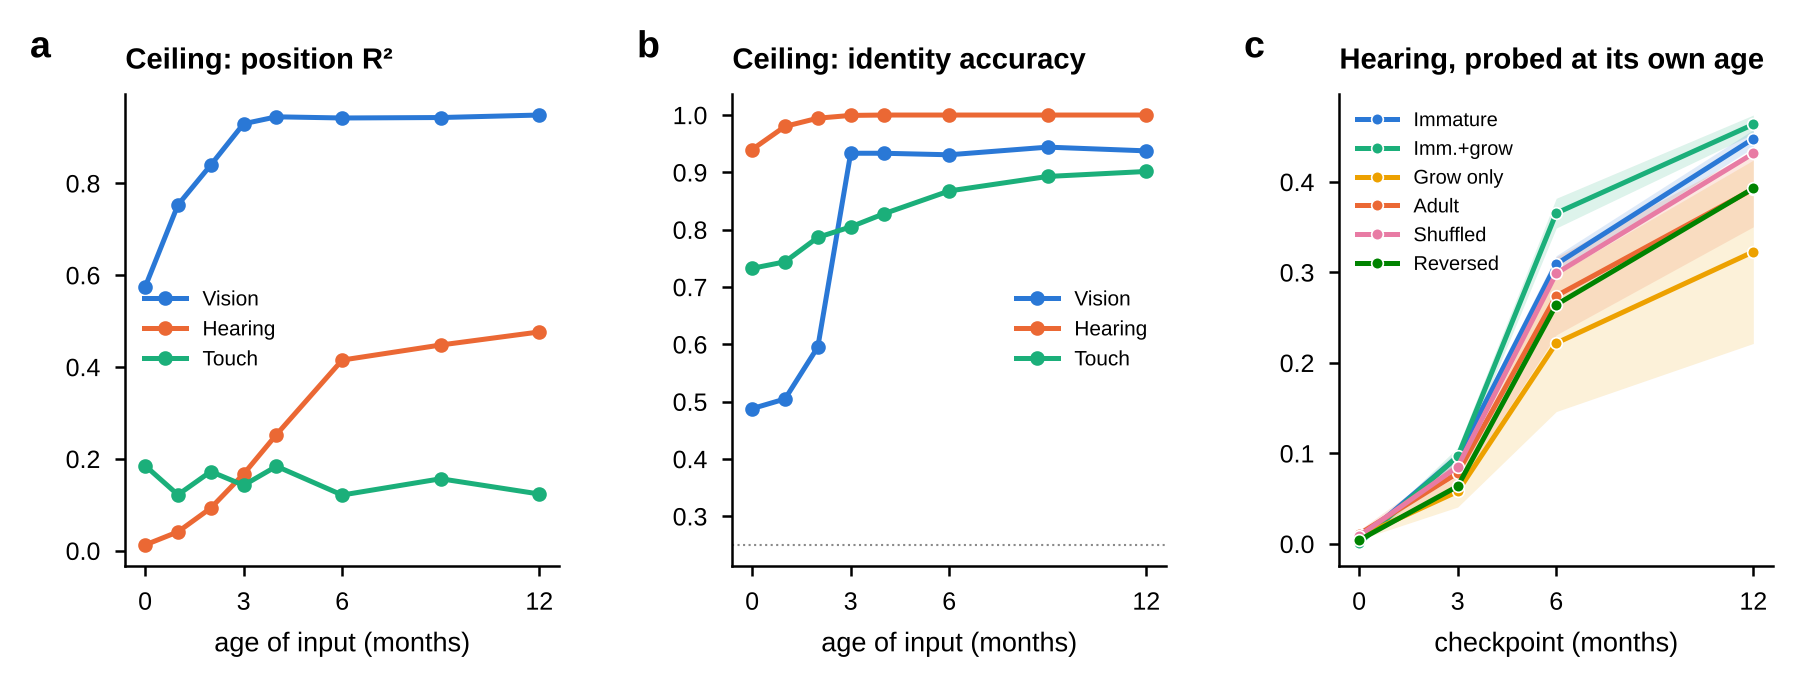
\includegraphics[width=\textwidth,height=0.78\textheight,keepaspectratio]{ed3_ceiling_ownage.png}
\caption{\textbf{Information ceilings and own-age probes.} \textbf{a}, \textbf{b}, Supervised ceilings per sense and age. \textbf{c}, Hearing probed on own-age input.}
\end{figure}


\printbibliography

\end{document}
